\section{Santa Fe laser Time series prediction}
The santa fe laser competition data stems from a 1989 paper, physicists measured the intensity of a unidirectional far infrared $NH_3$ laser\footnote{U. H\"{u}bner et al, Dimensions and entropies of chaotic intensity pulsations in a single-mode far-infrared NH3 laser, \url{http://journals.aps.org/pra/pdf/10.1103/PhysRevA.40.6354}}. In physics these types of lasers are modeled using so called Lorenz-Haken models. These models are chaotic systems, whith their Lyapunov exponent determining the speed by which trajectories starting a similar initial conditions diverge. In practice the quality any approximaiton made using Lorenz-Haken models depends on the of the initial conditions and the constants used in the model. 
\begin{figure}
\centering
\includegraphics[scale = 0.25]{../src/figure/origPaper.png}
% This file was created by matlab2tikz.
% Minimal pgfplots version: 1.3
%
%The latest updates can be retrieved from
%  http://www.mathworks.com/matlabcentral/fileexchange/22022-matlab2tikz
%where you can also make suggestions and rate matlab2tikz.
%
\documentclass[tikz]{standalone}
\usepackage{pgfplots}
\usepackage{grffile}
\pgfplotsset{compat=newest}
\usetikzlibrary{plotmarks}
\usepackage{amsmath}

\begin{document}
\definecolor{mycolor1}{rgb}{0.00000,0.44700,0.74100}%
%
\begin{tikzpicture}

\begin{axis}[%
width=1.5in,
height=1.5in,
scale only axis,
xmin=0,
xmax=1200,
ymin=0,
ymax=300
]
\addplot [color=mycolor1,solid,forget plot]
  table[row sep=crcr]{%
1	86\\
2	141\\
3	95\\
4	41\\
5	22\\
6	21\\
7	32\\
8	72\\
9	138\\
10	111\\
11	48\\
12	23\\
13	19\\
14	27\\
15	59\\
16	129\\
17	129\\
18	58\\
19	27\\
20	19\\
21	24\\
22	46\\
23	112\\
24	144\\
25	73\\
26	30\\
27	20\\
28	19\\
29	37\\
30	92\\
31	152\\
32	93\\
33	36\\
34	20\\
35	18\\
36	29\\
37	71\\
38	146\\
39	117\\
40	46\\
41	23\\
42	18\\
43	22\\
44	52\\
45	128\\
46	142\\
47	62\\
48	26\\
49	17\\
50	19\\
51	37\\
52	100\\
53	158\\
54	86\\
55	32\\
56	17\\
57	17\\
58	27\\
59	72\\
60	154\\
61	118\\
62	43\\
63	20\\
64	15\\
65	21\\
66	47\\
67	128\\
68	150\\
69	63\\
70	24\\
71	16\\
72	17\\
73	33\\
74	92\\
75	166\\
76	95\\
77	33\\
78	16\\
79	14\\
80	22\\
81	58\\
82	149\\
83	137\\
84	50\\
85	20\\
86	15\\
87	16\\
88	35\\
89	106\\
90	169\\
91	82\\
92	28\\
93	15\\
94	14\\
95	23\\
96	65\\
97	160\\
98	133\\
99	45\\
100	18\\
101	14\\
102	16\\
103	36\\
104	111\\
105	176\\
106	80\\
107	26\\
108	14\\
109	13\\
110	20\\
111	60\\
112	163\\
113	140\\
114	45\\
115	18\\
116	12\\
117	14\\
118	30\\
119	98\\
120	185\\
121	93\\
122	28\\
123	14\\
124	12\\
125	17\\
126	46\\
127	145\\
128	167\\
129	58\\
130	19\\
131	11\\
132	12\\
133	21\\
134	68\\
135	183\\
136	132\\
137	38\\
138	15\\
139	11\\
140	13\\
141	26\\
142	93\\
143	202\\
144	100\\
145	27\\
146	12\\
147	10\\
148	13\\
149	30\\
150	114\\
151	206\\
152	82\\
153	21\\
154	11\\
155	9\\
156	10\\
157	30\\
158	120\\
159	215\\
160	77\\
161	20\\
162	10\\
163	8\\
164	9\\
165	21\\
166	95\\
167	234\\
168	99\\
169	22\\
170	9\\
171	8\\
172	7\\
173	9\\
174	35\\
175	176\\
176	215\\
177	46\\
178	11\\
179	7\\
180	5\\
181	4\\
182	3\\
183	4\\
184	19\\
185	105\\
186	125\\
187	55\\
188	30\\
189	28\\
190	41\\
191	71\\
192	98\\
193	79\\
194	49\\
195	34\\
196	33\\
197	47\\
198	75\\
199	95\\
200	76\\
201	48\\
202	34\\
203	35\\
204	49\\
205	78\\
206	96\\
207	75\\
208	47\\
209	34\\
210	34\\
211	49\\
212	81\\
213	99\\
214	76\\
215	46\\
216	32\\
217	33\\
218	49\\
219	83\\
220	101\\
221	74\\
222	44\\
223	32\\
224	33\\
225	50\\
226	85\\
227	103\\
228	73\\
229	43\\
230	30\\
231	31\\
232	49\\
233	85\\
234	106\\
235	74\\
236	43\\
237	31\\
238	31\\
239	49\\
240	87\\
241	109\\
242	76\\
243	41\\
244	29\\
245	30\\
246	47\\
247	87\\
248	110\\
249	76\\
250	41\\
251	28\\
252	30\\
253	47\\
254	88\\
255	114\\
256	79\\
257	41\\
258	28\\
259	28\\
260	45\\
261	86\\
262	117\\
263	82\\
264	42\\
265	26\\
266	26\\
267	43\\
268	84\\
269	119\\
270	85\\
271	42\\
272	26\\
273	25\\
274	39\\
275	80\\
276	121\\
277	90\\
278	43\\
279	26\\
280	24\\
281	36\\
282	76\\
283	123\\
284	96\\
285	46\\
286	26\\
287	23\\
288	35\\
289	72\\
290	123\\
291	102\\
292	50\\
293	27\\
294	22\\
295	31\\
296	64\\
297	121\\
298	110\\
299	53\\
300	27\\
301	21\\
302	28\\
303	57\\
304	117\\
305	120\\
306	59\\
307	28\\
308	20\\
309	25\\
310	49\\
311	109\\
312	128\\
313	68\\
314	31\\
315	20\\
316	23\\
317	43\\
318	98\\
319	135\\
320	77\\
321	34\\
322	22\\
323	22\\
324	36\\
325	86\\
326	139\\
327	91\\
328	38\\
329	21\\
330	19\\
331	30\\
332	73\\
333	137\\
334	107\\
335	44\\
336	23\\
337	19\\
338	26\\
339	59\\
340	129\\
341	125\\
342	55\\
343	24\\
344	18\\
345	22\\
346	47\\
347	114\\
348	140\\
349	68\\
350	28\\
351	18\\
352	19\\
353	36\\
354	93\\
355	150\\
356	88\\
357	34\\
358	19\\
359	18\\
360	28\\
361	72\\
362	147\\
363	112\\
364	43\\
365	20\\
366	16\\
367	23\\
368	53\\
369	131\\
370	137\\
371	58\\
372	24\\
373	16\\
374	19\\
375	38\\
376	104\\
377	156\\
378	80\\
379	30\\
380	17\\
381	16\\
382	28\\
383	75\\
384	156\\
385	112\\
386	40\\
387	18\\
388	15\\
389	21\\
390	51\\
391	132\\
392	145\\
393	59\\
394	22\\
395	15\\
396	17\\
397	32\\
398	96\\
399	164\\
400	89\\
401	30\\
402	16\\
403	14\\
404	24\\
405	62\\
406	153\\
407	130\\
408	46\\
409	19\\
410	13\\
411	17\\
412	37\\
413	113\\
414	165\\
415	75\\
416	25\\
417	14\\
418	13\\
419	24\\
420	68\\
421	164\\
422	123\\
423	40\\
424	17\\
425	13\\
426	16\\
427	38\\
428	118\\
429	170\\
430	71\\
431	24\\
432	13\\
433	12\\
434	22\\
435	65\\
436	167\\
437	129\\
438	40\\
439	16\\
440	12\\
441	14\\
442	33\\
443	107\\
444	182\\
445	81\\
446	24\\
447	12\\
448	11\\
449	17\\
450	51\\
451	156\\
452	155\\
453	49\\
454	17\\
455	11\\
456	11\\
457	23\\
458	77\\
459	189\\
460	115\\
461	32\\
462	13\\
463	9\\
464	12\\
465	30\\
466	107\\
467	197\\
468	82\\
469	23\\
470	10\\
471	9\\
472	12\\
473	36\\
474	134\\
475	192\\
476	64\\
477	18\\
478	10\\
479	8\\
480	13\\
481	37\\
482	148\\
483	195\\
484	58\\
485	16\\
486	9\\
487	8\\
488	10\\
489	29\\
490	132\\
491	220\\
492	67\\
493	15\\
494	8\\
495	6\\
496	7\\
497	14\\
498	66\\
499	237\\
500	137\\
501	25\\
502	9\\
503	6\\
504	5\\
505	4\\
506	5\\
507	25\\
508	165\\
509	233\\
510	51\\
511	12\\
512	7\\
513	7\\
514	7\\
515	18\\
516	80\\
517	201\\
518	109\\
519	29\\
520	12\\
521	10\\
522	14\\
523	38\\
524	128\\
525	169\\
526	63\\
527	20\\
528	11\\
529	11\\
530	23\\
531	74\\
532	173\\
533	114\\
534	34\\
535	14\\
536	11\\
537	14\\
538	37\\
539	122\\
540	172\\
541	67\\
542	21\\
543	11\\
544	11\\
545	20\\
546	64\\
547	169\\
548	131\\
549	39\\
550	13\\
551	9\\
552	12\\
553	28\\
554	100\\
555	188\\
556	88\\
557	25\\
558	11\\
559	10\\
560	14\\
561	41\\
562	141\\
563	176\\
564	57\\
565	17\\
566	10\\
567	10\\
568	16\\
569	56\\
570	175\\
571	149\\
572	41\\
573	14\\
574	8\\
575	9\\
576	18\\
577	67\\
578	196\\
579	130\\
580	32\\
581	11\\
582	8\\
583	7\\
584	17\\
585	66\\
586	207\\
587	131\\
588	30\\
589	10\\
590	7\\
591	6\\
592	12\\
593	48\\
594	193\\
595	172\\
596	39\\
597	11\\
598	7\\
599	6\\
600	6\\
601	16\\
602	86\\
603	255\\
604	107\\
605	19\\
606	8\\
607	5\\
608	4\\
609	3\\
610	2\\
611	2\\
612	7\\
613	23\\
614	8\\
615	6\\
616	8\\
617	16\\
618	33\\
619	57\\
620	65\\
621	56\\
622	46\\
623	46\\
624	54\\
625	64\\
626	66\\
627	59\\
628	49\\
629	46\\
630	48\\
631	58\\
632	67\\
633	67\\
634	60\\
635	50\\
636	47\\
637	51\\
638	60\\
639	69\\
640	68\\
641	58\\
642	50\\
643	46\\
644	52\\
645	61\\
646	71\\
647	68\\
648	58\\
649	48\\
650	46\\
651	53\\
652	64\\
653	72\\
654	68\\
655	56\\
656	47\\
657	45\\
658	53\\
659	65\\
660	73\\
661	67\\
662	54\\
663	46\\
664	46\\
665	55\\
666	67\\
667	74\\
668	66\\
669	54\\
670	44\\
671	46\\
672	55\\
673	70\\
674	76\\
675	66\\
676	51\\
677	45\\
678	46\\
679	58\\
680	73\\
681	77\\
682	65\\
683	52\\
684	44\\
685	46\\
686	59\\
687	75\\
688	78\\
689	64\\
690	49\\
691	43\\
692	47\\
693	61\\
694	78\\
695	79\\
696	63\\
697	47\\
698	43\\
699	47\\
700	63\\
701	80\\
702	79\\
703	61\\
704	46\\
705	42\\
706	48\\
707	66\\
708	84\\
709	80\\
710	60\\
711	46\\
712	42\\
713	50\\
714	68\\
715	86\\
716	80\\
717	59\\
718	43\\
719	41\\
720	50\\
721	71\\
722	88\\
723	79\\
724	56\\
725	41\\
726	41\\
727	51\\
728	73\\
729	91\\
730	78\\
731	55\\
732	41\\
733	40\\
734	52\\
735	75\\
736	94\\
737	78\\
738	54\\
739	39\\
740	40\\
741	52\\
742	79\\
743	95\\
744	76\\
745	50\\
746	37\\
747	38\\
748	52\\
749	80\\
750	97\\
751	76\\
752	50\\
753	36\\
754	37\\
755	54\\
756	83\\
757	98\\
758	74\\
759	47\\
760	34\\
761	37\\
762	53\\
763	85\\
764	100\\
765	74\\
766	45\\
767	34\\
768	35\\
769	54\\
770	87\\
771	103\\
772	72\\
773	43\\
774	33\\
775	35\\
776	53\\
777	88\\
778	103\\
779	73\\
780	43\\
781	32\\
782	33\\
783	53\\
784	91\\
785	105\\
786	72\\
787	41\\
788	31\\
789	33\\
790	54\\
791	91\\
792	108\\
793	72\\
794	41\\
795	30\\
796	32\\
797	51\\
798	93\\
799	111\\
800	74\\
801	41\\
802	29\\
803	31\\
804	51\\
805	93\\
806	113\\
807	75\\
808	40\\
809	29\\
810	30\\
811	49\\
812	92\\
813	118\\
814	78\\
815	41\\
816	28\\
817	29\\
818	46\\
819	90\\
820	120\\
821	82\\
822	42\\
823	29\\
824	28\\
825	45\\
826	88\\
827	124\\
828	86\\
829	43\\
830	27\\
831	27\\
832	41\\
833	83\\
834	126\\
835	91\\
836	45\\
837	27\\
838	26\\
839	38\\
840	78\\
841	127\\
842	99\\
843	47\\
844	27\\
845	24\\
846	35\\
847	72\\
848	126\\
849	106\\
850	52\\
851	28\\
852	23\\
853	32\\
854	65\\
855	123\\
856	116\\
857	56\\
858	29\\
859	22\\
860	28\\
861	56\\
862	117\\
863	126\\
864	64\\
865	30\\
866	22\\
867	27\\
868	49\\
869	107\\
870	133\\
871	74\\
872	32\\
873	21\\
874	23\\
875	41\\
876	95\\
877	140\\
878	84\\
879	36\\
880	21\\
881	21\\
882	35\\
883	80\\
884	141\\
885	99\\
886	42\\
887	22\\
888	20\\
889	29\\
890	67\\
891	135\\
892	117\\
893	49\\
894	24\\
895	18\\
896	25\\
897	52\\
898	122\\
899	134\\
900	62\\
901	26\\
902	18\\
903	20\\
904	41\\
905	104\\
906	148\\
907	79\\
908	32\\
909	18\\
910	19\\
911	32\\
912	82\\
913	151\\
914	100\\
915	39\\
916	19\\
917	17\\
918	25\\
919	62\\
920	140\\
921	128\\
922	52\\
923	22\\
924	17\\
925	21\\
926	44\\
927	116\\
928	150\\
929	71\\
930	27\\
931	18\\
932	18\\
933	32\\
934	88\\
935	159\\
936	98\\
937	36\\
938	19\\
939	16\\
940	25\\
941	61\\
942	146\\
943	132\\
944	52\\
945	21\\
946	17\\
947	19\\
948	41\\
949	113\\
950	161\\
951	76\\
952	28\\
953	16\\
954	16\\
955	28\\
956	77\\
957	163\\
958	114\\
959	39\\
960	19\\
961	15\\
962	20\\
963	47\\
964	132\\
965	156\\
966	62\\
967	24\\
968	15\\
969	16\\
970	30\\
971	86\\
972	173\\
973	102\\
974	34\\
975	16\\
976	13\\
977	19\\
978	50\\
979	141\\
980	154\\
981	57\\
982	21\\
983	13\\
984	14\\
985	27\\
986	87\\
987	179\\
988	103\\
989	33\\
990	15\\
991	12\\
992	18\\
993	45\\
994	136\\
995	166\\
996	61\\
997	20\\
998	12\\
999	13\\
1000	23\\
1001	72\\
1002	178\\
1003	122\\
1004	36\\
1005	14\\
1006	11\\
1007	14\\
1008	32\\
1009	110\\
1010	188\\
1011	80\\
1012	23\\
1013	12\\
1014	10\\
1015	15\\
1016	45\\
1017	151\\
1018	169\\
1019	53\\
1020	18\\
1021	12\\
1022	9\\
1023	17\\
1024	60\\
1025	182\\
1026	143\\
1027	38\\
1028	13\\
1029	9\\
1030	9\\
1031	19\\
1032	71\\
1033	201\\
1034	126\\
1035	30\\
1036	12\\
1037	9\\
1038	8\\
1039	18\\
1040	70\\
1041	211\\
1042	131\\
1043	30\\
1044	11\\
1045	8\\
1046	8\\
1047	13\\
1048	47\\
1049	192\\
1050	179\\
1051	40\\
1052	13\\
1053	9\\
1054	7\\
1055	7\\
1056	14\\
1057	71\\
1058	255\\
1059	131\\
1060	24\\
1061	9\\
1062	7\\
1063	7\\
1064	5\\
1065	4\\
1066	3\\
1067	8\\
1068	20\\
1069	13\\
1070	10\\
1071	13\\
1072	20\\
1073	31\\
1074	42\\
1075	57\\
1076	68\\
1077	70\\
1078	59\\
1079	48\\
1080	46\\
1081	51\\
1082	61\\
1083	70\\
1084	67\\
1085	57\\
1086	48\\
1087	47\\
1088	53\\
1089	65\\
1090	72\\
1091	67\\
1092	57\\
1093	47\\
1094	47\\
1095	54\\
1096	67\\
1097	73\\
1098	66\\
1099	54\\
1100	48\\
1101	47\\
1102	55\\
1103	68\\
1104	74\\
1105	65\\
1106	54\\
1107	46\\
1108	48\\
1109	57\\
1110	70\\
1111	75\\
1112	65\\
1113	52\\
1114	45\\
1115	47\\
1116	58\\
1117	72\\
1118	74\\
1119	64\\
1120	50\\
1121	44\\
1122	47\\
1123	60\\
1124	74\\
1125	76\\
1126	63\\
1127	48\\
1128	44\\
1129	48\\
1130	61\\
1131	77\\
1132	77\\
1133	61\\
1134	48\\
1135	43\\
1136	48\\
1137	64\\
1138	79\\
1139	77\\
1140	60\\
1141	47\\
1142	42\\
1143	49\\
1144	67\\
1145	82\\
1146	77\\
1147	58\\
1148	45\\
1149	42\\
1150	51\\
1151	69\\
1152	84\\
1153	77\\
1154	56\\
1155	43\\
1156	42\\
1157	52\\
1158	72\\
1159	86\\
1160	77\\
1161	56\\
1162	42\\
1163	42\\
1164	54\\
1165	74\\
1166	88\\
1167	76\\
1168	54\\
1169	41\\
1170	42\\
1171	55\\
1172	78\\
1173	90\\
1174	75\\
1175	52\\
1176	41\\
1177	41\\
1178	56\\
1179	81\\
1180	92\\
1181	74\\
1182	51\\
1183	39\\
1184	42\\
1185	57\\
1186	83\\
1187	94\\
1188	72\\
1189	49\\
1190	38\\
1191	42\\
1192	58\\
1193	86\\
1194	95\\
1195	70\\
1196	47\\
1197	36\\
1198	40\\
1199	59\\
1200	89\\
};
\end{axis}
\end{tikzpicture}%
\end{document}
\caption{Data set measured by H\"{u}bner et al. and the subset selected for the Santa Fe competition.}
\label{fig:origAndSel}
\end{figure}
Figure~\ref{fig:origAndSel} shows a screenshot from the original paper and a plot of part of the measurements selected for the santa-fe competition. Instead of trying to figure out a good initial condition as well as reliable parameters for a Lorenz-Haken model a ls-svm in recurrent mode will be used to model this problem.
In the autonomous case of a recurrent model;
\begin{equation}
\hat{y}_k = f(\hat{y}_{k-1}, \hat{y}_{k-2}, \hat{y}_{k-3}, \dots)
\end{equation} 
a recurrent support vector machine can be used to model the system dynamics, given a starting value and windowed training data. Windowing the data means placing it into a Hankel matrix, where the rows represent shifted versions of the input. The ls-svm approach then uses the optimization problem: \footnote{Support Vector Machines: Methods and Applications, Suykens et al., page 225}
\begin{align}
\min\limits_{\mathbf{w},b,e} J_p(\mathbf{w},e) &= \frac{1}{2}\mathbf{w}^T \mathbf{w} + \gamma \frac{1}{2}\sum\limits_{k = p+1}^{p+N} e_k^2 \\
\text{such that } y_k - e_k &= \mathbf{w}^T \varphi(y_{k-1_k-p} - e_{k-1_k-p}) + b \;\;\; k = k \dots N.
\end{align}
The problem states that the approximation error $e_k  = y_k - \hat{y}_k$ should be reduced while enforcing the recurrent model dynamics. \\
\begin{figure}
\centering
% This file was created by matlab2tikz.
% Minimal pgfplots version: 1.3
%
%The latest updates can be retrieved from
%  http://www.mathworks.com/matlabcentral/fileexchange/22022-matlab2tikz
%where you can also make suggestions and rate matlab2tikz.
%
\documentclass[tikz]{standalone}
\usepackage{pgfplots}
\usepackage{grffile}
\pgfplotsset{compat=newest}
\usetikzlibrary{plotmarks}
\usepackage{amsmath}

\begin{document}
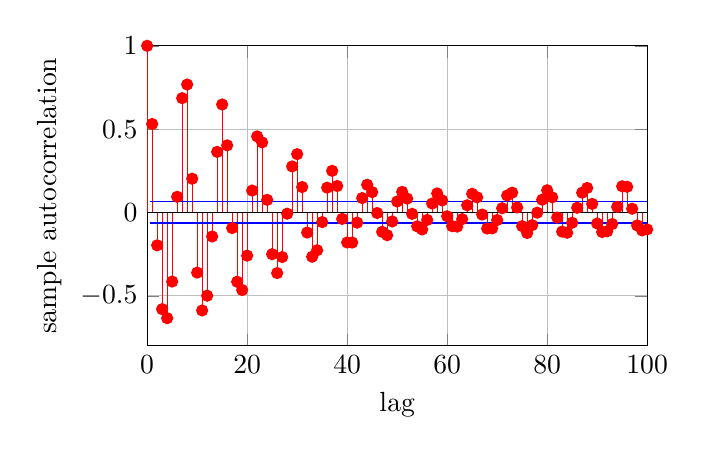
\begin{tikzpicture}

\begin{axis}[%
width=2.5in,
height=1.5in,
scale only axis,
xmin=0,
xmax=100,
xlabel={lag},
xmajorgrids,
ymin=-0.8,
ymax=1,
ylabel={sample autocorrelation},
ymajorgrids,
]
\addplot[ycomb,color=red,solid,mark size=2.0pt,mark=*,mark options={solid,fill=red}] plot table[row sep=crcr] {%
0	1\\
1	0.531012375277456\\
2	-0.19722744657221\\
3	-0.580093046226843\\
4	-0.634299361279394\\
5	-0.414510748215481\\
6	0.0940516998382318\\
7	0.685879732266424\\
8	0.767706341366509\\
9	0.202651503274669\\
10	-0.360753075814334\\
11	-0.587809692511437\\
12	-0.499374542532691\\
13	-0.144048742938735\\
14	0.363697338277312\\
15	0.647935296321381\\
16	0.402687846142643\\
17	-0.0936513180501337\\
18	-0.415641658040412\\
19	-0.465231628715779\\
20	-0.259047926027961\\
21	0.131616470574121\\
22	0.456403059036759\\
23	0.420665211089285\\
24	0.0757134794693025\\
25	-0.25029059785577\\
26	-0.363414909192172\\
27	-0.267448372946317\\
28	-0.00725311878350277\\
29	0.27641776758721\\
30	0.350147526867603\\
31	0.152519696142036\\
32	-0.120400195145866\\
33	-0.265388772684978\\
34	-0.226543296705639\\
35	-0.057524232662578\\
36	0.149038242145162\\
37	0.249893012712695\\
38	0.158918135972601\\
39	-0.0385093538827491\\
40	-0.17995280412447\\
41	-0.180326700511501\\
42	-0.0610913026777019\\
43	0.0864746394188238\\
44	0.166159947788355\\
45	0.122004495072026\\
46	-0.0033056106262259\\
47	-0.116431467216355\\
48	-0.136283669508414\\
49	-0.0538486021752314\\
50	0.0658938192822959\\
51	0.123492204764392\\
52	0.0833102007186009\\
53	-0.00824489146269923\\
54	-0.0832368116516709\\
55	-0.101938156163272\\
56	-0.0446236017196275\\
57	0.05381224724954\\
58	0.11444562311993\\
59	0.0723937663965338\\
60	-0.0226530416057325\\
61	-0.0821737593846169\\
62	-0.084963846753609\\
63	-0.0401676269139983\\
64	0.0432953457498929\\
65	0.112073757662789\\
66	0.0909093725544435\\
67	-0.0126049457164848\\
68	-0.0963090364883624\\
69	-0.0953149523683465\\
70	-0.0451934009589695\\
71	0.0254286808742385\\
72	0.101867891320578\\
73	0.118922313123251\\
74	0.0299211016844175\\
75	-0.0821706339376631\\
76	-0.123034935837922\\
77	-0.0760379895107557\\
78	-0.00119947423616588\\
79	0.0767222741387588\\
80	0.133366760645852\\
81	0.0907309328586872\\
82	-0.0303754385411401\\
83	-0.11484435701884\\
84	-0.121454231424134\\
85	-0.0615858654828823\\
86	0.0281677667722163\\
87	0.118911522175491\\
88	0.14719166655015\\
89	0.0513598687431599\\
90	-0.0661735316364488\\
91	-0.11720471472547\\
92	-0.112754441953474\\
93	-0.0693476056606004\\
94	0.0335169332028598\\
95	0.157044107441776\\
96	0.154067396062749\\
97	0.0226494900495964\\
98	-0.077591788580732\\
99	-0.107408975915327\\
100	-0.101719943568136\\
};
\addplot [color=blue,solid,forget plot]
  table[row sep=crcr]{%
0.5	0.0632455532033676\\
100	0.0632455532033676\\
};
\addplot [color=blue,solid,forget plot]
  table[row sep=crcr]{%
0.5	-0.0632455532033676\\
100	-0.0632455532033676\\
};
\addplot [color=black,solid,forget plot]
  table[row sep=crcr]{%
0	0\\
100	0\\
};
\end{axis}
\end{tikzpicture}%
\end{document}
\caption{Autocorrelation analysis of the training time-series shown with 95\% confidence bounds.}
\label{fig:santaFeAutocorr}
\end{figure}
In order to choose the window size the sample autocorrelation function shown in figure~\ref{fig:santaFeAutocorr} is considered. In the plot the autocorrelation values start to come close to the confidence bounds around a lag of fifty samples. Therefore a window size of fifty will be used as this shift covers the most significant samples. \\
\begin{figure}
\centering
\tikzset{mark size=1}
% This file was created by matlab2tikz.
% Minimal pgfplots version: 1.3
%
%The latest updates can be retrieved from
%  http://www.mathworks.com/matlabcentral/fileexchange/22022-matlab2tikz
%where you can also make suggestions and rate matlab2tikz.
%
\documentclass[tikz]{standalone}
\usepackage{pgfplots}
\usepackage{grffile}
\pgfplotsset{compat=newest}
\usetikzlibrary{plotmarks}
\usepackage{amsmath}

\begin{document}
\definecolor{mycolor1}{rgb}{0.00000,0.44700,0.74100}%
\definecolor{mycolor2}{rgb}{0.85000,0.32500,0.09800}%
\definecolor{mycolor3}{rgb}{0.92900,0.69400,0.12500}%
%
\begin{tikzpicture}

\begin{axis}[%
width=3.5in,
height=1.5in,
scale only axis,
xmin=0,
xmax=200,
ymin=0.0,
ymax=1
]
\addplot [color=mycolor1,solid,forget plot]
  table[row sep=crcr]{%
1	0.287937743190661\\
2	0.700389105058366\\
3	0.482490272373541\\
4	0.147859922178988\\
5	0.0622568093385214\\
6	0.0505836575875486\\
7	0.0622568093385214\\
8	0.132295719844358\\
9	0.43579766536965\\
10	0.739299610894942\\
11	0.319066147859922\\
12	0.0972762645914397\\
13	0.0544747081712062\\
14	0.0466926070038911\\
15	0.066147859922179\\
16	0.182879377431907\\
17	0.595330739299611\\
18	0.665369649805447\\
19	0.214007782101167\\
20	0.0778210116731518\\
21	0.0544747081712062\\
22	0.0428015564202335\\
23	0.0739299610894942\\
24	0.24124513618677\\
25	0.715953307392996\\
26	0.56420233463035\\
27	0.155642023346304\\
28	0.0583657587548638\\
29	0.0428015564202335\\
30	0.0428015564202335\\
31	0.0817120622568093\\
32	0.284046692607004\\
33	0.78988326848249\\
34	0.498054474708171\\
35	0.124513618677043\\
36	0.0544747081712062\\
37	0.0428015564202335\\
38	0.0389105058365759\\
39	0.0778210116731518\\
40	0.280155642023346\\
41	0.828793774319066\\
42	0.517509727626459\\
43	0.124513618677043\\
44	0.0505836575875486\\
45	0.0389105058365759\\
46	0.0389105058365759\\
47	0.0583657587548638\\
48	0.190661478599222\\
49	0.754863813229572\\
50	0.704280155642023\\
51	0.163424124513619\\
52	0.0583657587548638\\
53	0.0428015564202335\\
54	0.0350194552529183\\
55	0.0350194552529183\\
56	0.0622568093385214\\
57	0.284046692607004\\
58	1\\
59	0.517509727626459\\
60	0.101167315175097\\
61	0.0428015564202335\\
62	0.0350194552529183\\
63	0.0350194552529183\\
64	0.0272373540856031\\
65	0.0233463035019455\\
66	0.0194552529182879\\
67	0.0389105058365759\\
68	0.0856031128404669\\
69	0.0583657587548638\\
70	0.0466926070038911\\
71	0.0583657587548638\\
72	0.0856031128404669\\
73	0.1284046692607\\
74	0.171206225680934\\
75	0.229571984435798\\
76	0.272373540856031\\
77	0.280155642023346\\
78	0.237354085603113\\
79	0.194552529182879\\
80	0.186770428015564\\
81	0.206225680933852\\
82	0.245136186770428\\
83	0.280155642023346\\
84	0.268482490272374\\
85	0.229571984435798\\
86	0.194552529182879\\
87	0.190661478599222\\
88	0.214007782101167\\
89	0.260700389105058\\
90	0.287937743190661\\
91	0.268482490272374\\
92	0.229571984435798\\
93	0.190661478599222\\
94	0.190661478599222\\
95	0.217898832684825\\
96	0.268482490272374\\
97	0.291828793774319\\
98	0.264591439688716\\
99	0.217898832684825\\
100	0.194552529182879\\
101	0.190661478599222\\
102	0.221789883268482\\
103	0.272373540856031\\
104	0.295719844357977\\
105	0.260700389105058\\
106	0.217898832684825\\
107	0.186770428015564\\
108	0.194552529182879\\
109	0.229571984435798\\
110	0.280155642023346\\
111	0.299610894941634\\
112	0.260700389105058\\
113	0.21011673151751\\
114	0.182879377431907\\
115	0.190661478599222\\
116	0.233463035019455\\
117	0.287937743190661\\
118	0.295719844357977\\
119	0.256809338521401\\
120	0.202334630350195\\
121	0.178988326848249\\
122	0.190661478599222\\
123	0.24124513618677\\
124	0.295719844357977\\
125	0.303501945525292\\
126	0.252918287937743\\
127	0.194552529182879\\
128	0.178988326848249\\
129	0.194552529182879\\
130	0.245136186770428\\
131	0.307392996108949\\
132	0.307392996108949\\
133	0.245136186770428\\
134	0.194552529182879\\
135	0.175097276264591\\
136	0.194552529182879\\
137	0.256809338521401\\
138	0.315175097276265\\
139	0.307392996108949\\
140	0.24124513618677\\
141	0.190661478599222\\
142	0.171206225680934\\
143	0.198443579766537\\
144	0.268482490272374\\
145	0.326848249027237\\
146	0.307392996108949\\
147	0.233463035019455\\
148	0.182879377431907\\
149	0.171206225680934\\
150	0.206225680933852\\
151	0.276264591439689\\
152	0.334630350194553\\
153	0.307392996108949\\
154	0.22568093385214\\
155	0.175097276264591\\
156	0.171206225680934\\
157	0.21011673151751\\
158	0.287937743190661\\
159	0.342412451361868\\
160	0.307392996108949\\
161	0.22568093385214\\
162	0.171206225680934\\
163	0.171206225680934\\
164	0.217898832684825\\
165	0.295719844357977\\
166	0.350194552529183\\
167	0.303501945525292\\
168	0.217898832684825\\
169	0.167315175097276\\
170	0.171206225680934\\
171	0.221789883268482\\
172	0.311284046692607\\
173	0.357976653696498\\
174	0.299610894941634\\
175	0.21011673151751\\
176	0.167315175097276\\
177	0.167315175097276\\
178	0.22568093385214\\
179	0.32295719844358\\
180	0.365758754863813\\
181	0.295719844357977\\
182	0.206225680933852\\
183	0.159533073929961\\
184	0.171206225680934\\
185	0.229571984435798\\
186	0.330739299610895\\
187	0.373540856031128\\
188	0.287937743190661\\
189	0.198443579766537\\
190	0.155642023346304\\
191	0.171206225680934\\
192	0.233463035019455\\
193	0.342412451361868\\
194	0.377431906614786\\
195	0.280155642023346\\
196	0.190661478599222\\
197	0.147859922178988\\
198	0.163424124513619\\
199	0.237354085603113\\
200	0.35408560311284\\
};
\addplot [color=mycolor2,solid,forget plot]
  table[row sep=crcr]{%
1	0.290391387395838\\
2	0.701029557319766\\
3	0.483057043747828\\
4	0.154365637761923\\
5	0.0666086620113165\\
6	0.0501728269701258\\
7	0.0624047693455013\\
8	0.13432149654308\\
9	0.438107265537285\\
10	0.744097336941653\\
11	0.324895775106589\\
12	0.102278290803843\\
13	0.0556316238006404\\
14	0.050127620629275\\
15	0.0708298200621928\\
16	0.185080798125813\\
17	0.591094563213807\\
18	0.674939639698209\\
19	0.224785700746731\\
20	0.0739966714311767\\
21	0.0467375909063907\\
22	0.0465758575966532\\
23	0.076630277451799\\
24	0.239753486596926\\
25	0.708488176558831\\
26	0.585671527916416\\
27	0.16685390145932\\
28	0.0613533518889921\\
29	0.0439676966563466\\
30	0.0461910110167242\\
31	0.0808843476096627\\
32	0.274951461218364\\
33	0.770355553076368\\
34	0.536328451412344\\
35	0.134939099702276\\
36	0.0501031468178613\\
37	0.0394734293237683\\
38	0.0366351101993837\\
39	0.0712984899177717\\
40	0.254887084035749\\
41	0.787110303187066\\
42	0.584731318205248\\
43	0.136908530265657\\
44	0.0508296081752361\\
45	0.036702859947774\\
46	0.0305576987962545\\
47	0.04951090730705\\
48	0.160195465588631\\
49	0.638427556196384\\
50	0.855231279975158\\
51	0.205254071111674\\
52	0.0508091911443878\\
53	0.0368170542044121\\
54	0.0309329466286221\\
55	0.0268775608526285\\
56	0.0406079387272041\\
57	0.15736677480282\\
58	0.714186992968067\\
59	0.58968610233935\\
60	0.254497975013861\\
61	0.0423374968407262\\
62	0.00930888713924219\\
63	0.0101810712763414\\
64	0.0193496011420315\\
65	0.0749564180199652\\
66	0.0543161126177958\\
67	0.0348641836842875\\
68	0.219148410832293\\
69	0.163518183034531\\
70	0.0827454569449873\\
71	0.0702649019273583\\
72	0.106646726060072\\
73	0.173372056728336\\
74	0.27020161220009\\
75	0.355027426328402\\
76	0.298587655851796\\
77	0.163082649524849\\
78	0.160793786905344\\
79	0.200711546155201\\
80	0.250656568258795\\
81	0.290439503627947\\
82	0.317634032596406\\
83	0.257055921411974\\
84	0.19743198617071\\
85	0.158667869905126\\
86	0.201849201568171\\
87	0.249305994629114\\
88	0.288178529305654\\
89	0.309277723467985\\
90	0.263374582372061\\
91	0.194341910796043\\
92	0.171706366828728\\
93	0.202180218128379\\
94	0.254805526347611\\
95	0.302516813167252\\
96	0.300255038094762\\
97	0.253019369769928\\
98	0.201058781147157\\
99	0.181668461547233\\
100	0.201954525740478\\
101	0.258973774521654\\
102	0.316904893177288\\
103	0.313703752697108\\
104	0.243361788438698\\
105	0.196628722143247\\
106	0.189952118570169\\
107	0.210588025910655\\
108	0.269304665794855\\
109	0.325118259021932\\
110	0.303258888336713\\
111	0.230303509421868\\
112	0.182660458802993\\
113	0.18104095104289\\
114	0.212710171535161\\
115	0.278697077184316\\
116	0.333762172098188\\
117	0.299029089312531\\
118	0.229394272478611\\
119	0.183359082406352\\
120	0.178817313096002\\
121	0.214142866440125\\
122	0.28905652131744\\
123	0.342470315981969\\
124	0.301551300523095\\
125	0.220076546411602\\
126	0.179116876996908\\
127	0.176915114929046\\
128	0.219238452144026\\
129	0.298293189199546\\
130	0.351196645861553\\
131	0.296982139300177\\
132	0.214670795315536\\
133	0.171361038306001\\
134	0.175144988354055\\
135	0.222216014746566\\
136	0.308868831401286\\
137	0.357731466454167\\
138	0.292373910994868\\
139	0.206484371556811\\
140	0.166128391819814\\
141	0.172412060709784\\
142	0.225972625191485\\
143	0.319828753858112\\
144	0.363107002260094\\
145	0.287765999398907\\
146	0.199636997644854\\
147	0.161608959507855\\
148	0.170278743619969\\
149	0.231150322819538\\
150	0.33045175758305\\
151	0.369489752240588\\
152	0.281929438489484\\
153	0.193364935872142\\
154	0.15647211217402\\
155	0.168406723079809\\
156	0.234921639018199\\
157	0.341890180390998\\
158	0.374701518826543\\
159	0.276659500425492\\
160	0.185748165978849\\
161	0.151788215084416\\
162	0.166550679778251\\
163	0.238831600428427\\
164	0.352353083124605\\
165	0.378973627264565\\
166	0.271269755725509\\
167	0.179128421456343\\
168	0.147217123786929\\
169	0.164449217266604\\
170	0.242592736953792\\
171	0.362232775673046\\
172	0.383778262158739\\
173	0.266071063257028\\
174	0.17336933243557\\
175	0.142637663159083\\
176	0.162410807641045\\
177	0.245227281148023\\
178	0.372073852664147\\
179	0.388082972871163\\
180	0.262239413306324\\
181	0.167563125321007\\
182	0.138540861061359\\
183	0.159625729713699\\
184	0.247221168177362\\
185	0.380816590531905\\
186	0.393022464423036\\
187	0.259131572088633\\
188	0.162596325455562\\
189	0.134316473719436\\
190	0.156537707389075\\
191	0.247980427093435\\
192	0.388526216830554\\
193	0.39875059797291\\
194	0.257241752986229\\
195	0.158394607417351\\
196	0.130241502273668\\
197	0.153105153126653\\
198	0.247065410302028\\
199	0.395211481330239\\
200	0.405483560079441\\
};
\addplot [color=mycolor3,only marks,mark=*,mark options={solid},forget plot]
  table[row sep=crcr]{%
1	0.00245364420517624\\
2	0.000640452261400304\\
3	0.000566771374286679\\
4	0.00650571558293464\\
5	0.00435185267279509\\
6	0.000410830617422878\\
7	0.000147960006979864\\
8	0.00202577669872187\\
9	0.00230960016763559\\
10	0.00479772604671158\\
11	0.00582962724666702\\
12	0.00500202621240352\\
13	0.00115691562943412\\
14	0.00343501362538393\\
15	0.00468196014001386\\
16	0.00220142069390661\\
17	0.00423617608580429\\
18	0.00956998989276125\\
19	0.0107779186455634\\
20	0.003824340241975\\
21	0.00773711726481549\\
22	0.00377430117641976\\
23	0.00270031636230482\\
24	0.00149164958984466\\
25	0.00746513083416533\\
26	0.0214691932860657\\
27	0.0112118781130162\\
28	0.00298759313412829\\
29	0.0011661402361131\\
30	0.00338945459649072\\
31	0.000827714647146635\\
32	0.00909523138863993\\
33	0.0195277154061226\\
34	0.0382739767041725\\
35	0.0104254810252335\\
36	0.00437156135334496\\
37	0.00332812709646514\\
38	0.0022753956371922\\
39	0.00652252175538004\\
40	0.0252685579875978\\
41	0.0416834711320004\\
42	0.0672215905787893\\
43	0.0123949115886146\\
44	0.000245950587687491\\
45	0.00220764588880187\\
46	0.0083528070403214\\
47	0.00885485144781377\\
48	0.0304660130105909\\
49	0.116436257033188\\
50	0.150951124333134\\
51	0.0418299465980551\\
52	0.00755656761047598\\
53	0.00598450221582141\\
54	0.0040865086242962\\
55	0.0081418944002898\\
56	0.0216488706113173\\
57	0.126679917804184\\
58	0.285813007031933\\
59	0.0721763747128912\\
60	0.153330659838764\\
61	0.000464059579507278\\
62	0.0257105681136761\\
63	0.0248383839765769\\
64	0.00788775294357157\\
65	0.0516101145180197\\
66	0.0348608596995078\\
67	0.00404632215228837\\
68	0.133545297991826\\
69	0.105152424279667\\
70	0.0360528499410963\\
71	0.0118991431724945\\
72	0.0210436132196049\\
73	0.044967387467636\\
74	0.0989953865191559\\
75	0.125455441892605\\
76	0.0262141149957649\\
77	0.117072992498498\\
78	0.0765602986977686\\
79	0.00615901697232196\\
80	0.0638861402432308\\
81	0.0842138226940949\\
82	0.0724978458259784\\
83	0.0230997206113727\\
84	0.0710505041016634\\
85	0.0709041145306716\\
86	0.00729667238529119\\
87	0.0586445160298923\\
88	0.0741707472044869\\
89	0.0485773343629264\\
90	0.0245631608186009\\
91	0.0741405794763301\\
92	0.0578656176070692\\
93	0.0115187395291572\\
94	0.0641440477483893\\
95	0.0846179804824273\\
96	0.0317725478223888\\
97	0.0388094240043909\\
98	0.0635326585415593\\
99	0.036230371137592\\
100	0.00740199655759821\\
101	0.0683122959224323\\
102	0.0951150099088055\\
103	0.0413302118410766\\
104	0.0523580559192787\\
105	0.0640716669618119\\
106	0.0279467141146558\\
107	0.0238175978950906\\
108	0.0747521366119756\\
109	0.0955462745861347\\
110	0.0231032463133669\\
111	0.0693073855197666\\
112	0.0780399303020656\\
113	0.0290757804746195\\
114	0.0298307941032547\\
115	0.0880355985850944\\
116	0.100299137078733\\
117	0.01109134612187\\
118	0.0663255718793657\\
119	0.073450256115049\\
120	0.0235173172541921\\
121	0.0351545395918759\\
122	0.0983950427182183\\
123	0.101225179795198\\
124	0.00583145616511865\\
125	0.0834253991136899\\
126	0.0738014109408355\\
127	0.0176374142538329\\
128	0.040250125295777\\
129	0.103740660016667\\
130	0.106060459091125\\
131	0.0104108568087729\\
132	0.092722200793413\\
133	0.0737751484644269\\
134	0.0194075408288241\\
135	0.0471187384819745\\
136	0.114316302218406\\
137	0.100922127932767\\
138	0.0228011862813967\\
139	0.100908624552139\\
140	0.0751167443669566\\
141	0.0182494178894375\\
142	0.054766399510551\\
143	0.121385174091575\\
144	0.0946245119877206\\
145	0.0390822496283305\\
146	0.107755998464095\\
147	0.0718540755116003\\
148	0.0126006338119379\\
149	0.0599440971386045\\
150	0.124226076649198\\
151	0.093225160800899\\
152	0.0527009117050686\\
153	0.114028060236807\\
154	0.0692088216781196\\
155	0.00669055318478237\\
156	0.0637154133372649\\
157	0.131773448873488\\
158	0.0867637756358811\\
159	0.065752950936376\\
160	0.121644830130101\\
161	0.0738927187677245\\
162	0.00465554590268302\\
163	0.0676253747474931\\
164	0.13445425043978\\
165	0.0832537829065884\\
166	0.0789247968036734\\
167	0.124373524068949\\
168	0.0706817088978963\\
169	0.00286595783067273\\
170	0.0713865112728582\\
171	0.140442892404564\\
172	0.0724942154661322\\
173	0.0919055904394703\\
174	0.126241562506064\\
175	0.0674790683584267\\
176	0.00490436745623121\\
177	0.0779121060507466\\
178	0.146392918812007\\
179	0.0651257744275831\\
180	0.103519341557489\\
181	0.12815671903697\\
182	0.0676848198724934\\
183	9.26557837377107e-05\\
184	0.0760149424964286\\
185	0.151244606096107\\
186	0.0622831648121408\\
187	0.114409283942496\\
188	0.125341417735099\\
189	0.0641271060471014\\
190	0.000895684042771794\\
191	0.0767742014125011\\
192	0.155063181811099\\
193	0.0563381466110423\\
194	0.120190153628557\\
195	0.121761034605995\\
196	0.0604199763255536\\
197	0.00524523094766427\\
198	0.0836412857884095\\
199	0.157857395727126\\
200	0.0513979569666009\\
};
\end{axis}
\end{tikzpicture}%
\end{document}
% This file was created by matlab2tikz.
% Minimal pgfplots version: 1.3
%
%The latest updates can be retrieved from
%  http://www.mathworks.com/matlabcentral/fileexchange/22022-matlab2tikz
%where you can also make suggestions and rate matlab2tikz.
%
\documentclass[tikz]{standalone}
\usepackage{pgfplots}
\usepackage{grffile}
\pgfplotsset{compat=newest}
\usetikzlibrary{plotmarks}
\usepackage{amsmath}

\begin{document}
\definecolor{mycolor1}{rgb}{0.00000,0.44700,0.74100}%
\definecolor{mycolor2}{rgb}{0.85000,0.32500,0.09800}%
\definecolor{mycolor3}{rgb}{0.92900,0.69400,0.12500}%
%
\begin{tikzpicture}

\begin{axis}[%
width=3.5in,
height=1.5in,
scale only axis,
xmin=0,
xmax=200,
ymin=0,
ymax=1
]
\addplot [color=mycolor1,solid,forget plot]
  table[row sep=crcr]{%
1	0.287937743190661\\
2	0.700389105058366\\
3	0.482490272373541\\
4	0.147859922178988\\
5	0.0622568093385214\\
6	0.0505836575875486\\
7	0.0622568093385214\\
8	0.132295719844358\\
9	0.43579766536965\\
10	0.739299610894942\\
11	0.319066147859922\\
12	0.0972762645914397\\
13	0.0544747081712062\\
14	0.0466926070038911\\
15	0.066147859922179\\
16	0.182879377431907\\
17	0.595330739299611\\
18	0.665369649805447\\
19	0.214007782101167\\
20	0.0778210116731518\\
21	0.0544747081712062\\
22	0.0428015564202335\\
23	0.0739299610894942\\
24	0.24124513618677\\
25	0.715953307392996\\
26	0.56420233463035\\
27	0.155642023346304\\
28	0.0583657587548638\\
29	0.0428015564202335\\
30	0.0428015564202335\\
31	0.0817120622568093\\
32	0.284046692607004\\
33	0.78988326848249\\
34	0.498054474708171\\
35	0.124513618677043\\
36	0.0544747081712062\\
37	0.0428015564202335\\
38	0.0389105058365759\\
39	0.0778210116731518\\
40	0.280155642023346\\
41	0.828793774319066\\
42	0.517509727626459\\
43	0.124513618677043\\
44	0.0505836575875486\\
45	0.0389105058365759\\
46	0.0389105058365759\\
47	0.0583657587548638\\
48	0.190661478599222\\
49	0.754863813229572\\
50	0.704280155642023\\
51	0.163424124513619\\
52	0.0583657587548638\\
53	0.0428015564202335\\
54	0.0350194552529183\\
55	0.0350194552529183\\
56	0.0622568093385214\\
57	0.284046692607004\\
58	1\\
59	0.517509727626459\\
60	0.101167315175097\\
61	0.0428015564202335\\
62	0.0350194552529183\\
63	0.0350194552529183\\
64	0.0272373540856031\\
65	0.0233463035019455\\
66	0.0194552529182879\\
67	0.0389105058365759\\
68	0.0856031128404669\\
69	0.0583657587548638\\
70	0.0466926070038911\\
71	0.0583657587548638\\
72	0.0856031128404669\\
73	0.1284046692607\\
74	0.171206225680934\\
75	0.229571984435798\\
76	0.272373540856031\\
77	0.280155642023346\\
78	0.237354085603113\\
79	0.194552529182879\\
80	0.186770428015564\\
81	0.206225680933852\\
82	0.245136186770428\\
83	0.280155642023346\\
84	0.268482490272374\\
85	0.229571984435798\\
86	0.194552529182879\\
87	0.190661478599222\\
88	0.214007782101167\\
89	0.260700389105058\\
90	0.287937743190661\\
91	0.268482490272374\\
92	0.229571984435798\\
93	0.190661478599222\\
94	0.190661478599222\\
95	0.217898832684825\\
96	0.268482490272374\\
97	0.291828793774319\\
98	0.264591439688716\\
99	0.217898832684825\\
100	0.194552529182879\\
101	0.190661478599222\\
102	0.221789883268482\\
103	0.272373540856031\\
104	0.295719844357977\\
105	0.260700389105058\\
106	0.217898832684825\\
107	0.186770428015564\\
108	0.194552529182879\\
109	0.229571984435798\\
110	0.280155642023346\\
111	0.299610894941634\\
112	0.260700389105058\\
113	0.21011673151751\\
114	0.182879377431907\\
115	0.190661478599222\\
116	0.233463035019455\\
117	0.287937743190661\\
118	0.295719844357977\\
119	0.256809338521401\\
120	0.202334630350195\\
121	0.178988326848249\\
122	0.190661478599222\\
123	0.24124513618677\\
124	0.295719844357977\\
125	0.303501945525292\\
126	0.252918287937743\\
127	0.194552529182879\\
128	0.178988326848249\\
129	0.194552529182879\\
130	0.245136186770428\\
131	0.307392996108949\\
132	0.307392996108949\\
133	0.245136186770428\\
134	0.194552529182879\\
135	0.175097276264591\\
136	0.194552529182879\\
137	0.256809338521401\\
138	0.315175097276265\\
139	0.307392996108949\\
140	0.24124513618677\\
141	0.190661478599222\\
142	0.171206225680934\\
143	0.198443579766537\\
144	0.268482490272374\\
145	0.326848249027237\\
146	0.307392996108949\\
147	0.233463035019455\\
148	0.182879377431907\\
149	0.171206225680934\\
150	0.206225680933852\\
151	0.276264591439689\\
152	0.334630350194553\\
153	0.307392996108949\\
154	0.22568093385214\\
155	0.175097276264591\\
156	0.171206225680934\\
157	0.21011673151751\\
158	0.287937743190661\\
159	0.342412451361868\\
160	0.307392996108949\\
161	0.22568093385214\\
162	0.171206225680934\\
163	0.171206225680934\\
164	0.217898832684825\\
165	0.295719844357977\\
166	0.350194552529183\\
167	0.303501945525292\\
168	0.217898832684825\\
169	0.167315175097276\\
170	0.171206225680934\\
171	0.221789883268482\\
172	0.311284046692607\\
173	0.357976653696498\\
174	0.299610894941634\\
175	0.21011673151751\\
176	0.167315175097276\\
177	0.167315175097276\\
178	0.22568093385214\\
179	0.32295719844358\\
180	0.365758754863813\\
181	0.295719844357977\\
182	0.206225680933852\\
183	0.159533073929961\\
184	0.171206225680934\\
185	0.229571984435798\\
186	0.330739299610895\\
187	0.373540856031128\\
188	0.287937743190661\\
189	0.198443579766537\\
190	0.155642023346304\\
191	0.171206225680934\\
192	0.233463035019455\\
193	0.342412451361868\\
194	0.377431906614786\\
195	0.280155642023346\\
196	0.190661478599222\\
197	0.147859922178988\\
198	0.163424124513619\\
199	0.237354085603113\\
200	0.35408560311284\\
};
\addplot [color=mycolor2,solid,forget plot]
  table[row sep=crcr]{%
1	0.291886869228443\\
2	0.697130726731448\\
3	0.487799517158665\\
4	0.154774877019776\\
5	0.0649354193559451\\
6	0.0494689776532875\\
7	0.0622211250534412\\
8	0.133790172612665\\
9	0.439045015501186\\
10	0.741296755625048\\
11	0.324459566114609\\
12	0.104504614984293\\
13	0.0553617505128097\\
14	0.0495722203999687\\
15	0.0701554166143887\\
16	0.18540737023975\\
17	0.588806323031377\\
18	0.681674407410467\\
19	0.218943319946057\\
20	0.0722517312762941\\
21	0.0454905216331989\\
22	0.0466996782981562\\
23	0.07590612017735\\
24	0.240824815754049\\
25	0.702525346705381\\
26	0.596658586733029\\
27	0.161894653061468\\
28	0.0616341779215883\\
29	0.0433290672730867\\
30	0.0452146367491821\\
31	0.0802024024926485\\
32	0.276353732989184\\
33	0.761039308806729\\
34	0.554968094478045\\
35	0.132778254832576\\
36	0.0513670936443507\\
37	0.0384154601938425\\
38	0.0364137827996357\\
39	0.0707994850994975\\
40	0.256014874444811\\
41	0.761981244166447\\
42	0.621590404190769\\
43	0.143252736104326\\
44	0.0509496210753744\\
45	0.0363653806427595\\
46	0.0301100343214265\\
47	0.0492643271850693\\
48	0.156905881495576\\
49	0.598403051948812\\
50	0.879675355297601\\
51	0.229833508816847\\
52	0.0537787267090907\\
53	0.0360416918114368\\
54	0.0285121116569129\\
55	0.0280485373213473\\
56	0.0371421695182688\\
57	0.158970393570298\\
58	0.630413455946958\\
59	0.578609832904323\\
60	0.315254080824035\\
61	0.0530594721829632\\
62	0.0106088775040281\\
63	0.0150289680166378\\
64	0.0260390889042243\\
65	0.094725792111361\\
66	0.0885148473395054\\
67	0.0969655099947817\\
68	0.328561586133897\\
69	0.219766029762373\\
70	0.104172820171157\\
71	0.0830862103737487\\
72	0.124668003269277\\
73	0.194547025526097\\
74	0.286557076498616\\
75	0.389930128544149\\
76	0.371572614563561\\
77	0.164191783085857\\
78	0.140188650686886\\
79	0.179935943578036\\
80	0.239265956551433\\
81	0.298210826561904\\
82	0.352478654507743\\
83	0.316713010608256\\
84	0.242856129897474\\
85	0.142212198387658\\
86	0.170220282232791\\
87	0.22307911836009\\
88	0.284374100528503\\
89	0.337545618750158\\
90	0.313531819131156\\
91	0.243671476623087\\
92	0.174463554111852\\
93	0.16478514226028\\
94	0.217985461527671\\
95	0.290014834145011\\
96	0.323686802806832\\
97	0.302512810257594\\
98	0.254000765964999\\
99	0.198247679185648\\
100	0.168548364601543\\
101	0.207004958208068\\
102	0.296239784700953\\
103	0.340261237366632\\
104	0.295720166677682\\
105	0.247554192280746\\
106	0.219694377319942\\
107	0.189752322151385\\
108	0.211345525025351\\
109	0.290779162152801\\
110	0.340784669309231\\
111	0.291804234813182\\
112	0.231799055608591\\
113	0.205384152875912\\
114	0.199991495167201\\
115	0.225728650952047\\
116	0.290436754187828\\
117	0.333368290430046\\
118	0.306374474346272\\
119	0.23698713191375\\
120	0.199334067766042\\
121	0.200362215331887\\
122	0.236623255888904\\
123	0.2942221411035\\
124	0.335271925860197\\
125	0.302708262506278\\
126	0.238849581078997\\
127	0.197053395169444\\
128	0.1976554720901\\
129	0.238362278536101\\
130	0.302204902590099\\
131	0.335557143406162\\
132	0.300387383168526\\
133	0.234249353104478\\
134	0.196058268946134\\
135	0.196971073659317\\
136	0.239961146649698\\
137	0.307897659807763\\
138	0.337595224220046\\
139	0.294791876844628\\
140	0.230019686908917\\
141	0.194366612290787\\
142	0.19747164893116\\
143	0.242806492024891\\
144	0.311770989826536\\
145	0.340476013543803\\
146	0.289526567860604\\
147	0.224551871520425\\
148	0.192277816996463\\
149	0.199831644010913\\
150	0.247053202537272\\
151	0.316942573220909\\
152	0.341853724083972\\
153	0.285065515976205\\
154	0.218569427452066\\
155	0.189302928245652\\
156	0.200605300576123\\
157	0.251986428887872\\
158	0.323470141053304\\
159	0.342875858999844\\
160	0.279753954963934\\
161	0.213284887386943\\
162	0.186682343556792\\
163	0.20066766003998\\
164	0.256722802471902\\
165	0.330169697096791\\
166	0.343455242047821\\
167	0.27315902677445\\
168	0.208158573561525\\
169	0.184343635808928\\
170	0.201479297918338\\
171	0.261302052239579\\
172	0.33713052661746\\
173	0.343133103885865\\
174	0.266833618355779\\
175	0.202690621255063\\
176	0.18191067914461\\
177	0.202363557121287\\
178	0.266750869283501\\
179	0.343749936528164\\
180	0.342478793635838\\
181	0.260183967232131\\
182	0.197434083783726\\
183	0.179303292357947\\
184	0.203324147022125\\
185	0.27253588923457\\
186	0.35049690180924\\
187	0.341077220827622\\
188	0.253615055559763\\
189	0.192292089438201\\
190	0.176642391843989\\
191	0.204363887233555\\
192	0.27851476786999\\
193	0.357389373720835\\
194	0.339000718225207\\
195	0.247180582725258\\
196	0.187322149608605\\
197	0.174097962990502\\
198	0.205333210683501\\
199	0.284704190037119\\
200	0.364113234179249\\
};
\addplot [color=mycolor3,only marks,mark=*,mark options={solid},forget plot]
  table[row sep=crcr]{%
1	0.00394912603778175\\
2	0.00325837832691755\\
3	0.00530924478512451\\
4	0.00691495484078772\\
5	0.0026786100174237\\
6	0.00111467993426116\\
7	3.56842850801897e-05\\
8	0.00149445276830687\\
9	0.00324735013153615\\
10	0.0019971447301067\\
11	0.00539341825468709\\
12	0.0072283503928534\\
13	0.000887042341603472\\
14	0.00287961339607762\\
15	0.00400755669220972\\
16	0.00252799280784313\\
17	0.00652441626823375\\
18	0.0163047576050193\\
19	0.00493553784488976\\
20	0.0055692803968577\\
21	0.00898418653800728\\
22	0.00389812187792278\\
23	0.00197615908785585\\
24	0.000420320432721305\\
25	0.0134279606876146\\
26	0.032456252102679\\
27	0.0062526297151641\\
28	0.00326841916672445\\
29	0.0005275108528532\\
30	0.00241308032894859\\
31	0.00150965976416083\\
32	0.00769295961782035\\
33	0.0288439596757611\\
34	0.0569136197698733\\
35	0.00826463615553324\\
36	0.00310761452685557\\
37	0.00438609622639101\\
38	0.00249672303694021\\
39	0.00702152657365426\\
40	0.0241407675785357\\
41	0.0668125301526197\\
42	0.10408067656431\\
43	0.0187391174272831\\
44	0.000365963487825763\\
45	0.00254512519381636\\
46	0.00880047151514937\\
47	0.00910143156979452\\
48	0.0337555971036458\\
49	0.15646076128076\\
50	0.175395199655578\\
51	0.0664093843032284\\
52	0.00458703204577314\\
53	0.00675986460879661\\
54	0.0065073435960054\\
55	0.00697091793157102\\
56	0.0251146398202526\\
57	0.125076299036706\\
58	0.369586544053042\\
59	0.0611001052778639\\
60	0.214086765648938\\
61	0.0102579157627297\\
62	0.0244105777488902\\
63	0.0199904872362805\\
64	0.00119826518137879\\
65	0.0713794886094155\\
66	0.0690595944212174\\
67	0.0580550041582059\\
68	0.24295847329343\\
69	0.161400271007509\\
70	0.0574802131672664\\
71	0.0247204516188849\\
72	0.0390648904288101\\
73	0.0661423562653964\\
74	0.115350850817682\\
75	0.160358144108352\\
76	0.0991990737075296\\
77	0.11596385893749\\
78	0.0971654349162266\\
79	0.0146165856048437\\
80	0.0524955285358687\\
81	0.0919851456280521\\
82	0.107342467737315\\
83	0.0365573685849095\\
84	0.0256263603748992\\
85	0.0873597860481396\\
86	0.0243322469500885\\
87	0.0324176397608682\\
88	0.0703663184273353\\
89	0.0768452296450994\\
90	0.0255940759404943\\
91	0.0248110136492866\\
92	0.0551084303239455\\
93	0.0258763363389415\\
94	0.0273239829284494\\
95	0.0721160014601856\\
96	0.055204312534459\\
97	0.0106840164832749\\
98	0.0105906737237165\\
99	0.0196511534991769\\
100	0.0260041645813363\\
101	0.0163434796088461\\
102	0.0744499014324705\\
103	0.0678876965106005\\
104	3.22319705481355e-07\\
105	0.013146196824312\\
106	0.00179554463511686\\
107	0.00298189413582034\\
108	0.0167929958424718\\
109	0.0612071777170037\\
110	0.0606290272858845\\
111	0.0078066601284526\\
112	0.0289013334964672\\
113	0.00473257864159729\\
114	0.0171121177352944\\
115	0.0350671723528257\\
116	0.0569737191683729\\
117	0.0454305472393841\\
118	0.0106546299882949\\
119	0.0198222066076506\\
120	0.00300056258415227\\
121	0.0213738884836384\\
122	0.0459617772896819\\
123	0.0529770049167292\\
124	0.03955208150222\\
125	0.000793683019014058\\
126	0.0140687068587463\\
127	0.00250086598656454\\
128	0.0186671452418511\\
129	0.0438097493532213\\
130	0.0570687158196706\\
131	0.0281641472972125\\
132	0.00700561294042346\\
133	0.0108868336659504\\
134	0.00150573976325427\\
135	0.0218737973947259\\
136	0.0454086174668187\\
137	0.0510883212863618\\
138	0.0224201269437811\\
139	0.0126011192643215\\
140	0.0112254492778533\\
141	0.00370513369156558\\
142	0.0262654232502264\\
143	0.0443629122583538\\
144	0.043288499554162\\
145	0.0136277645165659\\
146	0.017866428248345\\
147	0.00891116349902987\\
148	0.00939843956455683\\
149	0.0286254183299794\\
150	0.0408275216034195\\
151	0.0406779817812206\\
152	0.00722337388941907\\
153	0.0223274801327447\\
154	0.00711150640007452\\
155	0.0142056519810607\\
156	0.0293990748951888\\
157	0.0418696973703626\\
158	0.035532397862643\\
159	0.000463407637975866\\
160	0.0276390411450156\\
161	0.0123960464651971\\
162	0.0154761178758579\\
163	0.0294614343590465\\
164	0.0388239697870769\\
165	0.0344498527388144\\
166	0.00673931048136173\\
167	0.0303429187508419\\
168	0.00974025912329968\\
169	0.0170284607116522\\
170	0.0302730722374045\\
171	0.0395121689710964\\
172	0.0258464799248534\\
173	0.0148435498106328\\
174	0.0327772765858552\\
175	0.00742611026244661\\
176	0.0145955040473342\\
177	0.0350483820240106\\
178	0.041069935431361\\
179	0.0207927380845839\\
180	0.0232799612279752\\
181	0.0355358771258461\\
182	0.00879159715012576\\
183	0.0197702184279858\\
184	0.0321179213411909\\
185	0.0429639047987719\\
186	0.0197576021983447\\
187	0.0324636352035062\\
188	0.0343226876308986\\
189	0.00615149032833645\\
190	0.0210003684976855\\
191	0.0331576615526211\\
192	0.0450517328505352\\
193	0.0149769223589671\\
194	0.0384311883895788\\
195	0.032975059298088\\
196	0.00333932899061684\\
197	0.0262380408115136\\
198	0.0419090861698823\\
199	0.0473501044340059\\
200	0.0100276310664088\\
};
\end{axis}
\end{tikzpicture}%
\end{document}
\caption{Recurrent ls-svm approxmation of scaled Santa-Fee using the automatically found hyper-parameters $\gamma =  158.5795, \sigma^2 = 23.35559$ (top) and $\gamma = 75.4764, \sigma^2 = 27.7826$ (bottom) . The blue curve shows the validation data set, the red one the svm-approximation. Yellow dots indicate the error at any given point.}
\label{fig:santaFe}
\end{figure}
 Figure~\ref{fig:santaFe} shows recurrent svm approximation using automatically tuned hyper-parameters found trough a coupled simulated annealing, simplex optimization algorithm pair. Cross-validation was used in order to evaluate the  absolute error cost function. Results using this cost function have been significantly better then using a mean square error function or infinity norm based cost.   
      


\section{Changing window committee nets.}